The data handling is organised into 3 sections: The first being a MongoDB data-store for handling all the incoming data from the flowers, the second being the dashboard for visualising the data available in the data-store and the last being a central server that communicates with a lora-module via serial-port, parsing and saving the lora packets and also acting as a web-server to the dashboard.

\subsection{MongoDB Data store}
% Quick intro to MongoDB (No-SQL)
MongoDB is a No-SQL database that provides an expressive query language and flexible data-store that allows iteration of data models. It is a highly efficient database that supports millions of operations per sec and can handle petabytes of data as well being able to scale (grow) horizontally with support for database clusters.

% Benefits of MongoDB (Rapid prototyping)
This rich feature set provided us with a strong foundation as a data-store for the sunflowers for two main reasons. Firstly, during the development stage, it provided us with a medium for rapid prototyping as we were able to rapidly change the schema of the data that was being stored and 
% Scalability and distributed nature which can support distributed sunflowers
due the distributed and highly scalable nature of MongoDB; It is theoretically possible for us to scale this data-store to support thousands of sunflowers.

\subsection{Dashboard}
% Brief intro to the dashboard as a valuable tool for analytics
The dashboard acts as an operator user-interface for navigating the data in the MongoDB data-store. One of the functionalities we encoded into it is support for analytics on the Sun flower data, this is illustrated in figure \ref{figure:home} where we aggregated data on the temperature and humidity.
\begin{figure}
	\centering
	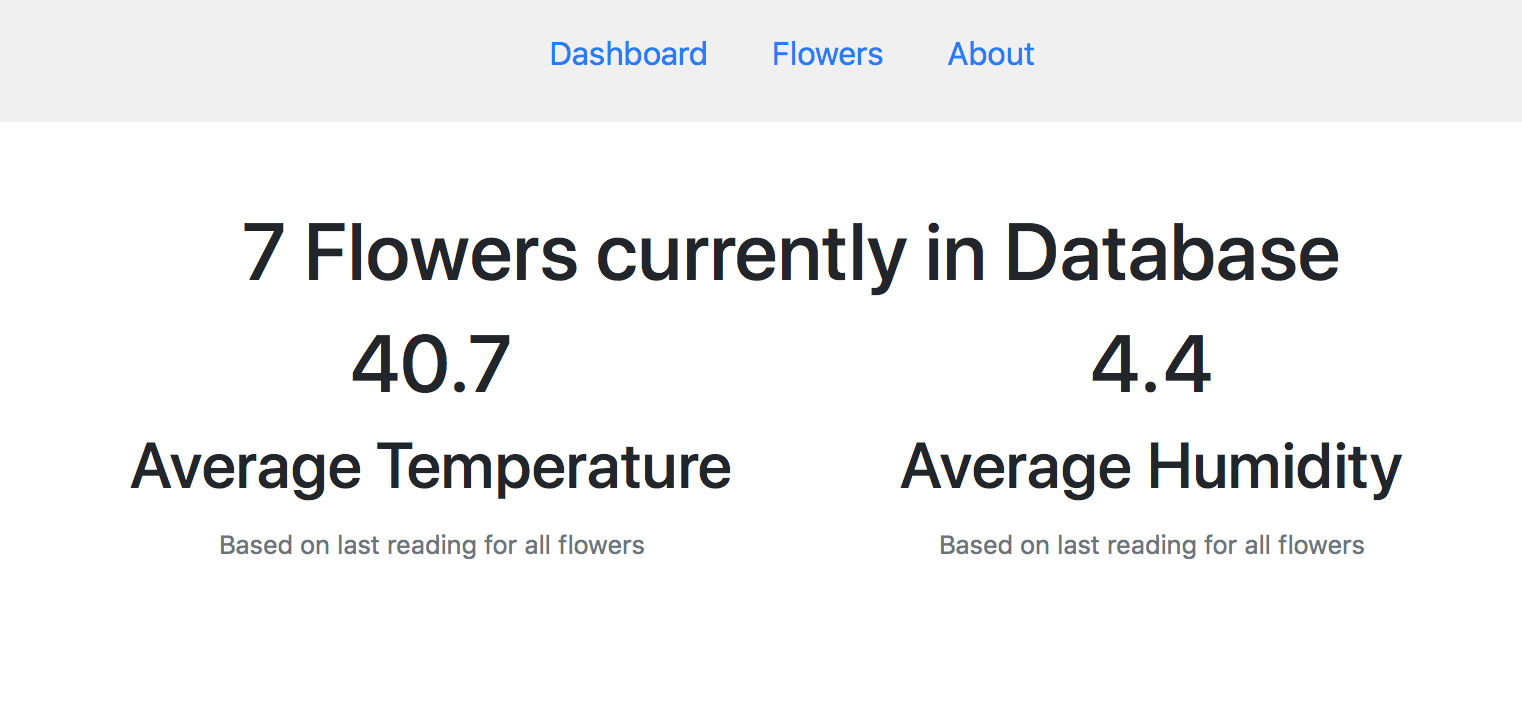
\includegraphics[width=\linewidth]{home}
	\caption{Homepage for the dashboard}
	\label{figure:home}
\end{figure}
\begin{figure}
	\centering
	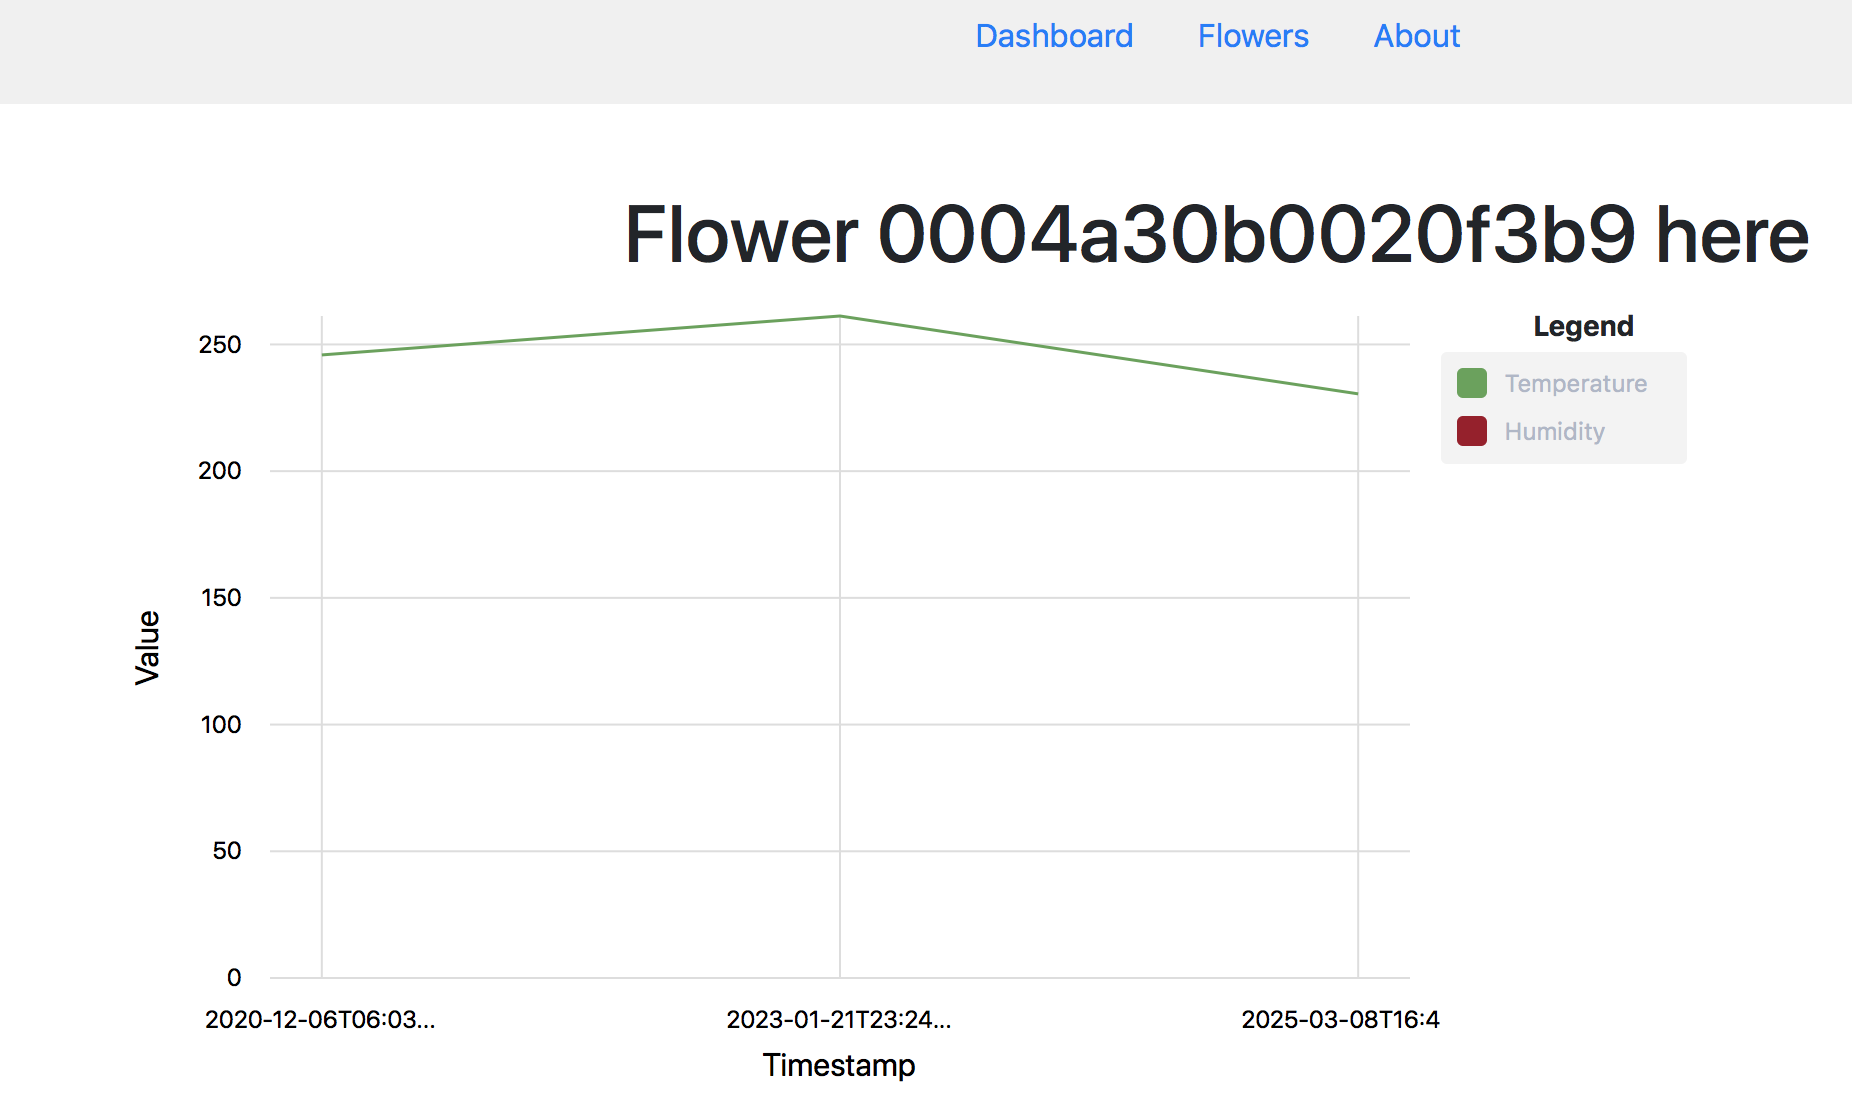
\includegraphics[width=\linewidth]{flowers}
	\caption{Sample detail page for a SunFlower}
	\label{figure:flower}
\end{figure}

% Quick intro into the tech behind the dashboard
The dashboard is built using web-technologies of which are \href{www.angular.io}{AngularJS} for the architecture and \href{https://swimlane.github.io/ngx-charts/}{Ngx-Charts} for the visualisations. The dashboard supports single-page apps and by default offline mode; highlighting the strong technologies used for the project.

% Currently supports one way communication i.e Flower => Server => Dashboard but support for bilateral comms could be added in the future
Currently the dashboard only receives data from the central server as data currently flows from the sun-flowers to the server and then to the dashboard. In the future, bilateral communication could be added; In figure \ref{figure:flower}, the sample page for a sun-flower is shown there, a sample feature that could be added would be a button to shutdown the flower where this command propagates from the dashboard to the central server and then to the sun-flower.



\subsection{Central Server}
% Quick intro in the tech behind the server (highly scalable and asynchronous in nature)
The central server is the main entry point for the data processing end. It is built using NodeJS, a highly scalable technology with first class asynchronous support; This is useful for our application where the packets are streamed as they arrive into the central server.

% Functionality of the server: Node serial port communication and parsing, saving to disk, processing the data for analytics
The pipeline of the central server from parsing the data to sending it to clients is described below and figure \ref{figure:arch} shows the flow of data across the entire application from the lora modem to the dashboard client.
\begin{itemize}
	\item The first thing the server does is to connect to the lora-modem via serial port and instructs it to listen for data packets from the flowers. It should be noted that the entire setup is asynchronous and data is just streamed into the server once it arrives.
	\item the central server receives it from the modem and parses it. The parsing is done with the assumption that the bits are stored in big endian format; Once this is completed, they are automatically saved into the MongoDB database where they update the data for an existing flower or create a store if the data is from a new flower.
\end{itemize} 

% REST API exposed which can be used by mobile apps, web-apps etc
The server exposes a REST(Representational State Transfer) API that enables it to communicate with any client that supports this protocol. For this project, we have built a dashboard app for the web that uses REST to communicate with the server but this could easily be adapted for another client such as an iOS mobile app. 
As the central server has a medium for communicating with the sun-flowers via the attached lora model, it is technically possible to enable the server pass commands on the flowers as mentioned earlier.

\begin{figure}
	\centering
	\includegraphics[width=\linewidth]{arch}
	\caption{Pipeline flow of data across the application}
	\label{figure:arch}
\end{figure}

%TODO: Include an image of the entire pipeline